
\section{Simulación de contagio en hospitales}

\subsection{Objetivo}

Dada la complejidad de Repast HPC y el tiempo disponible de la materia
para llevar a cabo el proyecto, se optó por priorizar el paralelismo en
la simulación, realizando mediciones de rendimiento y buscando posibles
mejoras. Por este motivo en la simulación solo se mantuvo una lógica de
transmisión entre los agentes, desplazándose de manera aleatoria sobre
un mapa trivial con paredes en los bordes, solo con el objetivo de
verificar que el modelo funciona correctamente y que los mapas y agentes
son generados de forma correcta (se considera que se brindan las
herramientas necesarias para profundizar en la lógica de la simulación
si se desea).

\subsection{Rendimiento}

Para realizar métricas de rendimiento, se ejecuta reiteradas veces la
simulación combinando distintos parámetros como el tamaño del mapa, la
cantidad de agentes y la distribución del mapa en cantidad de procesos.

De cada combinación realizada se mide el tiempo de ejecución para la
simulación con esas características.

\begin{figure}[H]
	\centering
	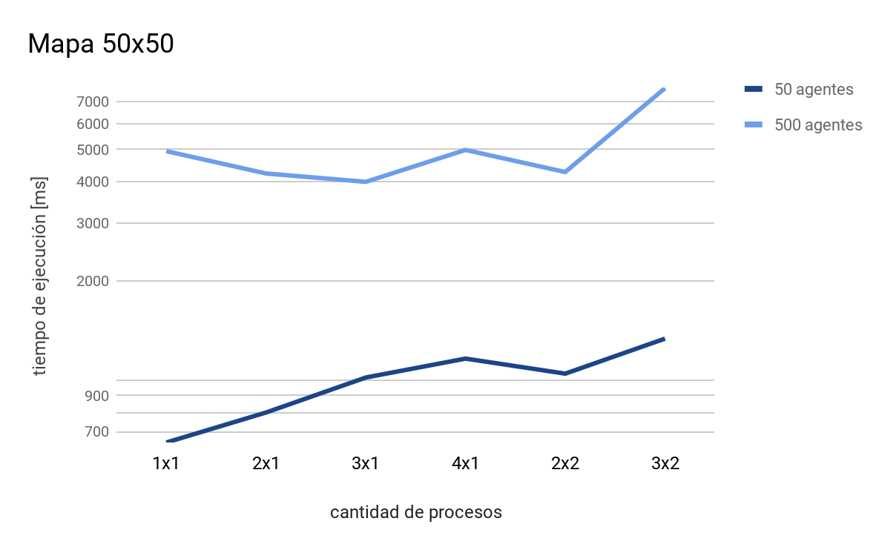
\includegraphics{Rendimiento1.png}
	\caption{Mapa de 50x50 con 50 y 500 Agentes}
\end{figure}

\begin{figure}[H]
	\centering
	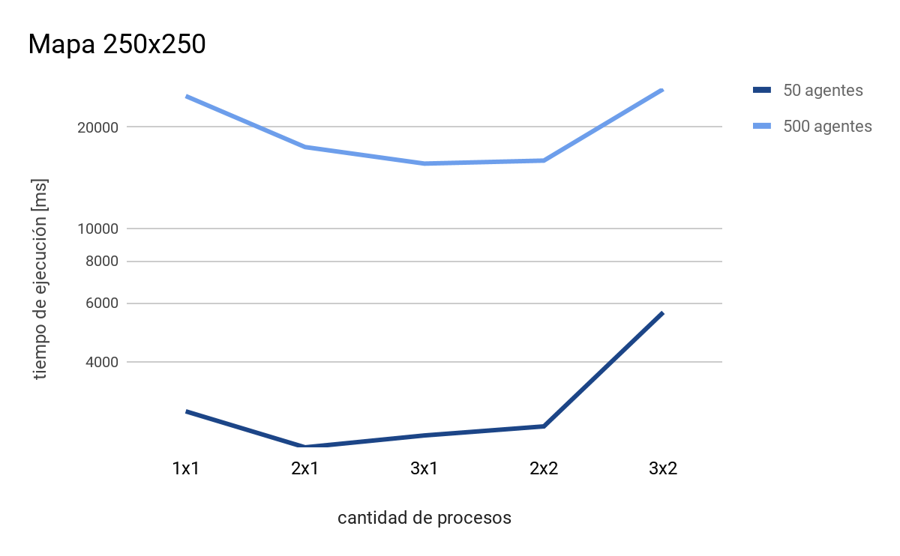
\includegraphics{Rendimiento2.png}
	\caption{Mapa de de 250x250 con 50 y 500 Agentes}
\end{figure}

Como podemos observar, cuando la proyección espacial se trata de un mapa
de tamaño reducido con poca o mediana cantidad de agentes, el
rendimiento no se ve favorecido al aumentar la cantidad de procesos,
sino al contrario, el tiempo de ejecución aumenta, debido al incremento
de comunicación; reduciendo el rendimiento del sistema.

En los siguientes casos, cuando el mapa espacial aumenta a un tamaño de
500x500, sí se puede observar una notable mejora de rendimiento cuando
se ejecuta la simulación en 1 y en 4 procesos, reduciendo el tiempo de
ejecución a aproximadamente la mitad al aumentar el grado de
paralelismo.

\begin{figure}[H]
	\centering
	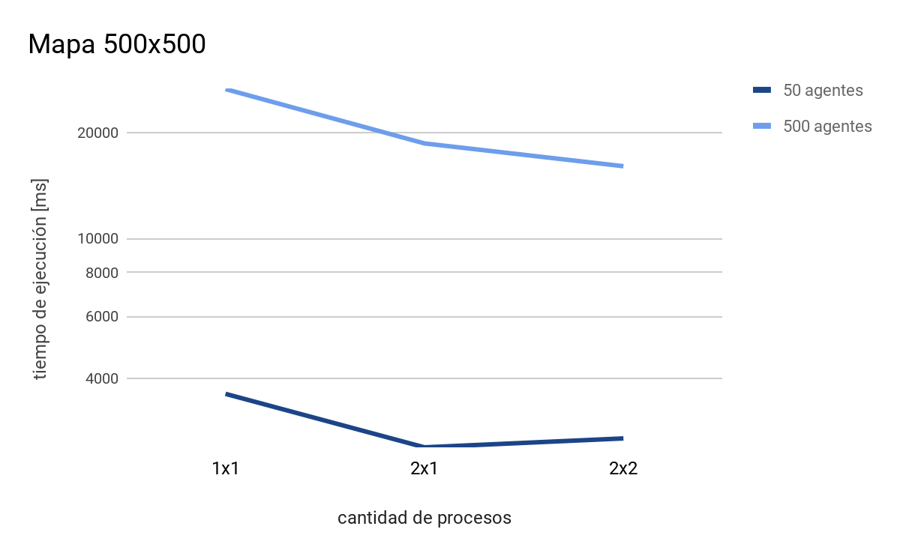
\includegraphics{Rendimiento3.png}
	\caption{Mapa de 500x500 con 50 y 500 agentes}
\end{figure}

\begin{figure}[H]
	\centering
	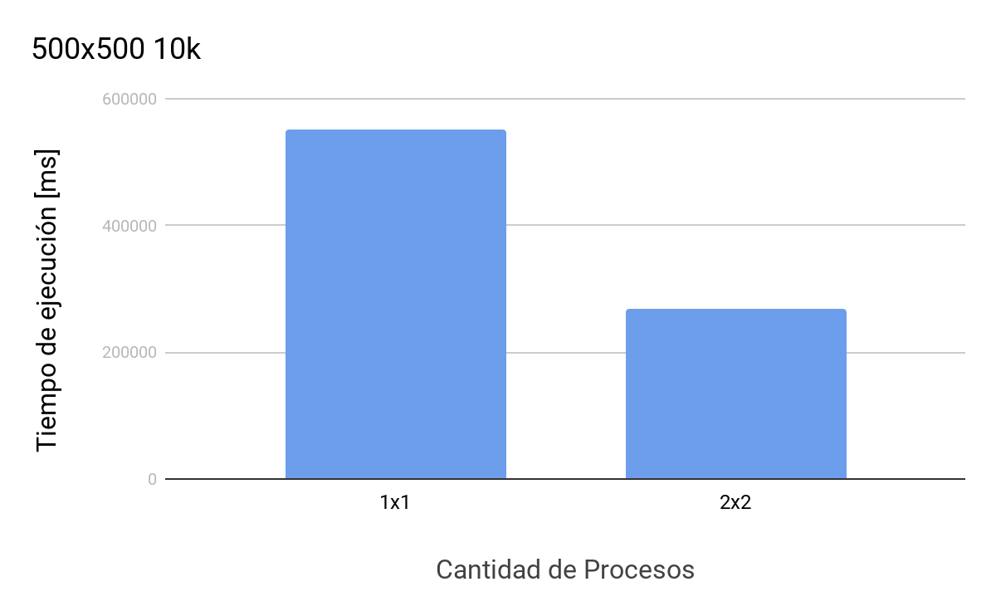
\includegraphics{Rendimiento4.png}
	\caption{Mapa de 500x500 con 10'000 agentes}
\end{figure}

\vspace{1\linewidth}

Estos resultados obtenidos se deben a que cuando el nivel de
procesamiento es reducido, la comunicación entre procesos es
excesivamente alta. Por lo que, tratándose de simulaciones que no
demandan un gran procesamiento, no se justifica la paralelización, ya
que el rendimiento no solo no mejorará, sino que se verá afectado, y a
su vez, la complejidad es mucho mayor. Por el contrario, cuando se trata
de simulaciones con una cantidad de agentes mayor, en un espacio
extenso, las mejoras en tiempo de ejecución son muy significativas,
reduciendo el mismo, en algunos casos, a casi el 50\%.

También, es necesario destacar otro factor que influye directamente en
el rendimiento de la simulación que es el balance de procesamiento para
cada proceso. Es decir, si la simulación se ejecuta, por ejemplo, en 4
procesos, el escenario perfecto sería que cada proceso ejecute el 25\%
del procesamiento total. De otra manera, todos los procesos tendrían que
esperarse entre sí, simulando una barrera, hasta que terminen su parte
de la ejecución. Luego, el scheduler puede realizar la sincronización
entre los mismos antes del siguiente tick, y así, que todos comiencen la
ejecución en el mismo instante.
